\section{Ejercicio 8}

\subsection{Implementación de Round Robin 2}

\indent Como nos indicaba la consigna de este ejercicio, se implementó un algoritmo Round Robin que no permite migración.\\
\indent A la hora de implementarlo, nos valimos de varias estructuras de datos que nos permitiesen de alguna manera hacer un seguimiento de la tareas, para saber cual será la próxima a ejecutarse.\\
\indent Una cola de tareas llamada $procesos$, donde encolamos las tareas que todavía no tienen un core asignado. Un vector de colas llamado $colas$, de tamaño igual a la cantidad de cores. En la posición $i$ de dicho vector encontramos la cola de tareas que fueron asignadas al core $i$. El vector $cores$ , de tamaño igual a la cantidad de cores del sistema. En la posicion $i$ de $cores$ se encuentra el pid de la tarea que está corriendo actualmente en el core $i$.\\
\indent Además, tenemos el diccionario $blockedProc$, donde guardaremos el core asignado a una tarea bloqueada.\\

\indent Cuando se carga una tarea, se la asigna al primer core libre que encuentre y se la agrega a su correspondiente cola. Si estuviesen todos ocupados, se la manda a la cola $procesos$.\\
\indent Siempre que un core deba realizar un cambio de tarea, ya sea porque la que estaba corriendo consumió su quantum, o porque se bloqueó o porque finalizó, se prioriza a las tareas que todavía no fueron asignadas a algún core por sobre las que tiene dicho core asignado. Esto es porque según nuestra implementación, si una tarea está en la cola de un core entonces fue corrida por lo menos una vez en ese core y además no está en la cola $procesos$.\\
\indent Si se encontrase un elemento en $procesos$ se la saca dicha cola y se la agrega a la cola del cpu correspondiente de manera tal que sea la próxima en salir en ser desencolada.Si no hubiese más elementos en $procesos$ entonces se prosigue con la siguiente tarea de la cola y dependiendo de si se terminó el quantum de la tarea que había estado corriendo en ese tick, se la encola al final de la cola correspondiente a su core, o se simplemente se la saca de allí.\\
\indent Si una tarea se bloquease, se la define en el diccionario con su correpondiente core de clave y se la quita de la cola de ese core. Cuando se desbloquee, se obtiene el core que tiene asignado del diccionario y la borra del diccionario.\\
\indent Una vez definidas todas las tareas en cada core, el funcionamiento del algoritmo es similar a pensar un round robin común y corriente para cada core.\\


\subsection{Experimentación}

\indent Se experimentó principalmente con el siguiente lote de tareas:\\


\indent TaskBatch 10 5\\


\indent TaskBatch 10 2\\


\indent TaskBatch 10 4\\


\indent TaskBatch 10 3\\


\indent TaskBatch 10 7\\

\indent Se estudiaron casos de uno, dos y tres cores. Para los casos multicore, se analizó qué ocurría cuando todos los cores tenían valores de quantum iguales y luego, algunos casos con distintos valores de quantum para cada core.\\

\indent Una primera hipótesis que se conjeturó antes de experimentar fue que mientras más cores hubiese más rápido se terminarían de ejecutar todas las tareas. Además, intuitivamente pensamos que a partir de cierto valor de quantum no habría diferencia en ni en la forma ni el tiempo de ejecución de la tareas.\\
\indent Es importante destacar que el valor de los quantum seguramente impacte en el core al que será asignado una tarea, puesto que puede ocurrir que con un quantum chico una tarea deje de correr y el cpu agarre otra sin core asignado, mientras que con un quantum más grande quizá la tarea se hubiera quedado ejecutando y no se asignara esa nueva tarea al core.\\
\indent Además, hay que destacar que si bien el algoritmo Round Robin 2 se ahorra de alguna manera pagar los costos de migración, podría ocurrir también que al no permitir migrar tareas de core, un core tenga muchas tareas asignadas mientras que otros están vacíos (ya sea porque las que corría se terminaron o están bloqueadas), y lo lógico sería usar dicho core para ejecutar otra tarea.\\
\indent Queremos observar que existe un cierto valor de quantum para cada core a partir del cual ya no se mejora el tiempo de ejecución de todas las tareas, aunque es de notar que dicho valor también dependerá del lote de tareas a correr.\\

\subsubsection{Un Core}

\indent Lo más destacable del estudio de este caso es que se comporta igual que un Round Robin común y corriente (y es lo esperable).\\
\indent Las conclusiones de la consigna anterior valen entonces para este caso. Para ello, se provee el gráfico con un quantum igual a ocho, que es el valor de quantum donde se estabilizaba el Round Robin con un core:\\

\begin{figure}[h]
	\centering                                                       
	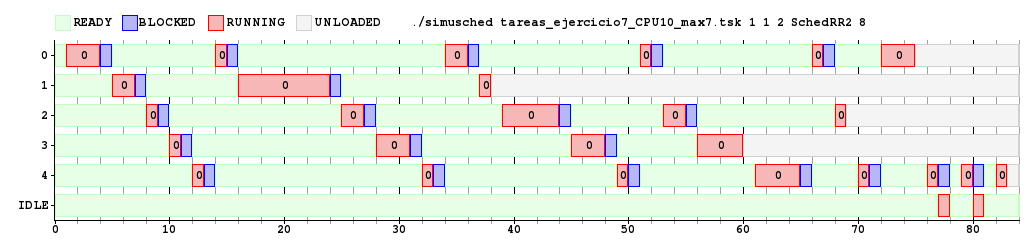
\includegraphics[width=450pt]{./figs/ej8/ej8-q8.png}
\end{figure}

\subsubsection{Dos Cores}

\indent Analicemos primero cuando ambos cores tiene el mismo quantum. Se estudiaron casos con quantums desde dos hasta diez. A partir de ellos se analizó el turnaround time y el waiting time de cada tarea.\\
\indent Veamos algunos gráficos que nos parecen sirven para ejemplificar:

\begin{figure}[h]
	\centering                                                       
	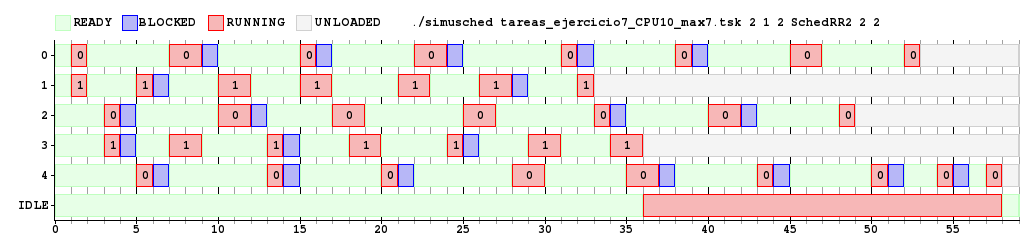
\includegraphics[width=450pt]{./figs/ej8/ej8-c2-q2.png}
\end{figure}


\begin{figure}[h]
	\centering                                                       
	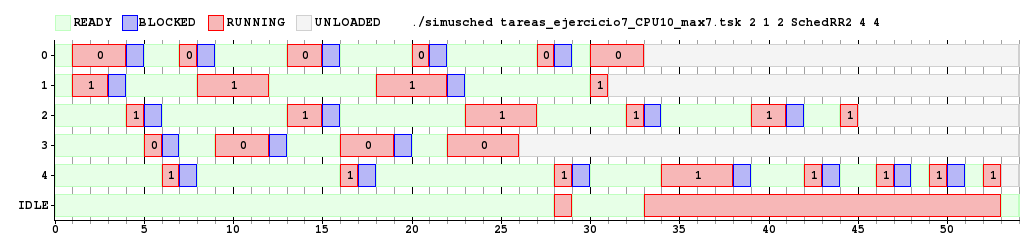
\includegraphics[width=450pt]{./figs/ej8/ej8-c2-q4.png}
\end{figure}


\indent Entre estos dos gráficos se observa como cambiando los quantum de 2 a 4 el cpu asigna las tareas de manera distinta. Se puede observar como en el primer caso la tarea 2 se ejecuta en el core 0 y en el segundo caso se ejecuta en el core 1. Algo similar ocurre con las tareas 3 y 4. Además, se observa como se terminan de ejecutar todas las tareas más rápido en este último caso.\\

\begin{figure}[h]
	\centering                                                       
	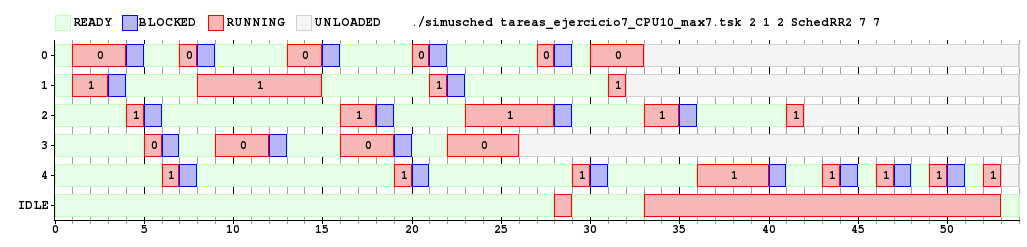
\includegraphics[width=450pt]{./figs/ej8/ej8-c2-q7.png}
\end{figure}

\begin{figure}[h]
	\centering                                                       
	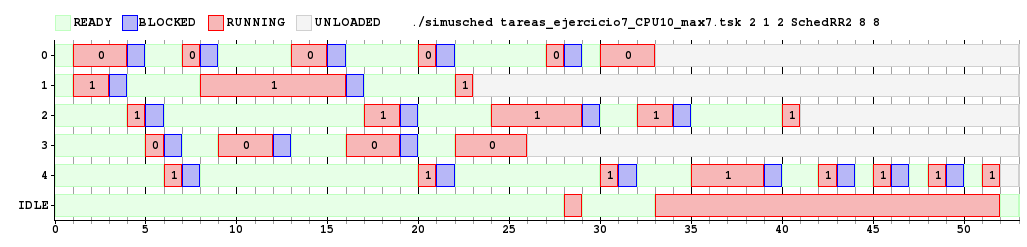
\includegraphics[width=450pt]{./figs/ej8/ej8-c2-q8.png}
\end{figure}

\begin{figure}[h]
\centering                                                       
	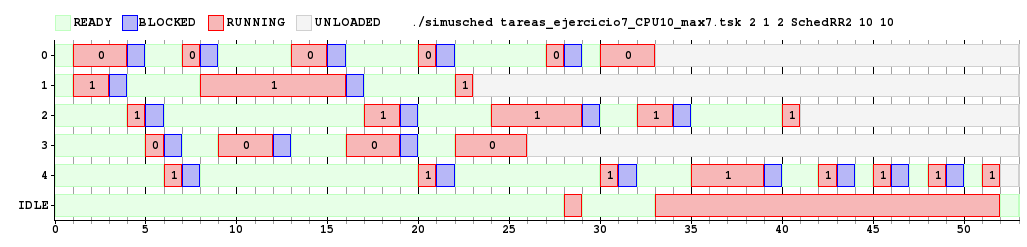
\includegraphics[width=450pt]{./figs/ej8/ej8-c2-q10.png}
\end{figure}

\indent Como ocurría en el caso de un core, observamos como a partir del caso con quantum igual a ocho, el scheduler actúa de la misma manera. Además en estos casos se observa como terminan de ejecutar todas las tareas más rápido que con quantum igual a cuatro.\\

\indent A partir de todos los casos de este tipo estudiados, se produjeron los siguientes gráficos que muestran la evolución del turnaround time y el waiting time de cada tarea en función del quantum utilizado:\\
\clearpage

\begin{figure}[h]
	\centering                                                       
	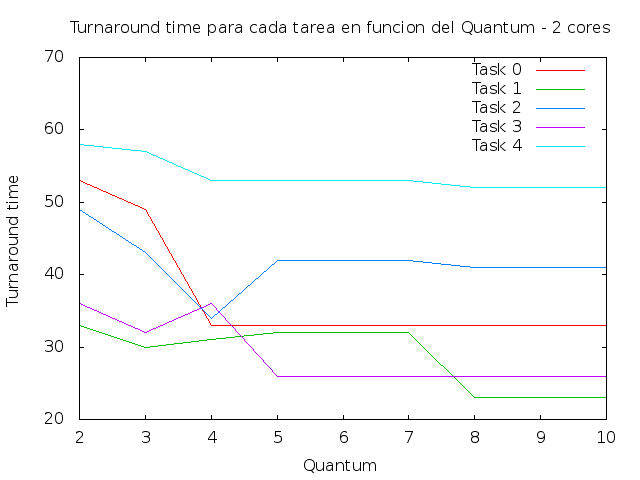
\includegraphics[width=280pt]{./figs/ej8/turnaroundtime2cores.png}
\end{figure}

\begin{figure}[h]
	\centering                                                       
	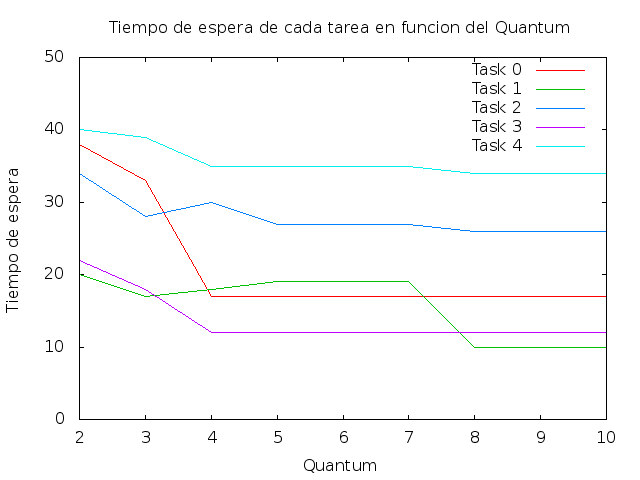
\includegraphics[width=280pt]{./figs/ej8/waitingTime2cores.png}
\end{figure}


\indent En tales gráficos se observa como en general el waiting time parece evolucionar de manera decreciente, a pesar de algunas pequeñas subidas en el gráfico hasta que se estabiliza para todas las tareas para un quantum igual a ocho (para algunas lo hace antes).\\
\indent En cuanto al turnaround time, es notable cómo también se estabiliza a partir del quantum igual a ocho, aunque se observa que es mucho más fluctuante. Es notable como la Task 4, que es la que más tarda en ejecutarse se termina de ejecutar más rápido a medida que se aumenta el quantum.\\


\indent Veamos el caso con quantums distintos. Aquí se analizaron menos casos. A partir de los casos con igual quantum por core, se observó que a partir de cierto quantum (distinto para cada core) las tareas que corrían en ese eran ejecutadas de la misma manera. Por ello, conjeturamos que quizá para cada core exista un quantum distinto que implicase que las todas tareas se correran de la manera más rápida (es decir equivalente al quantum igual a ocho cuando ambos tienen el mismo core).\\


\clearpage

\begin{figure}[h]	
	\centering                                                       
	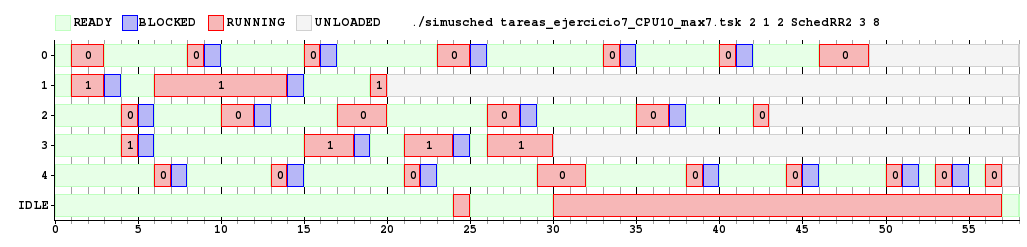
\includegraphics[width=450pt]{./figs/ej8/ej8-c2-q3-8.png}
\end{figure}

\begin{figure}[h]
	\centering                                                       
	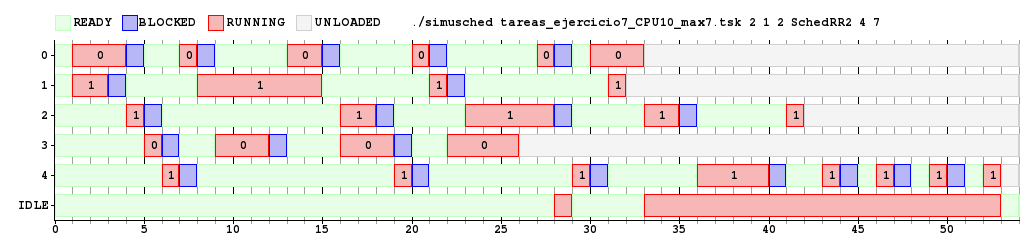
\includegraphics[width=450pt]{./figs/ej8/ej8-c2-q4-7.png}
\end{figure}

\begin{figure}[h]
	\centering                                                       
	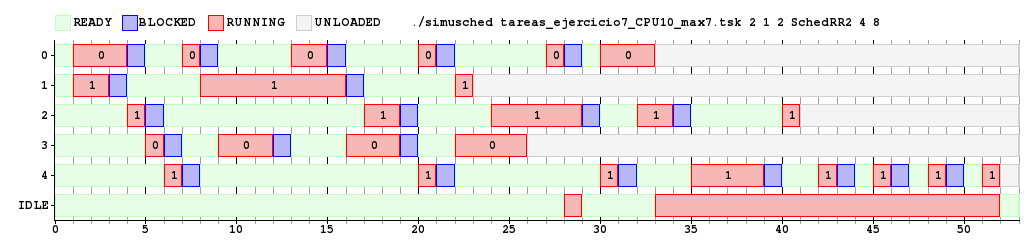
\includegraphics[width=450pt]{./figs/ej8/ej8-c2-q4-8.png}
\end{figure}

\begin{figure}[h]
\centering                                                       
	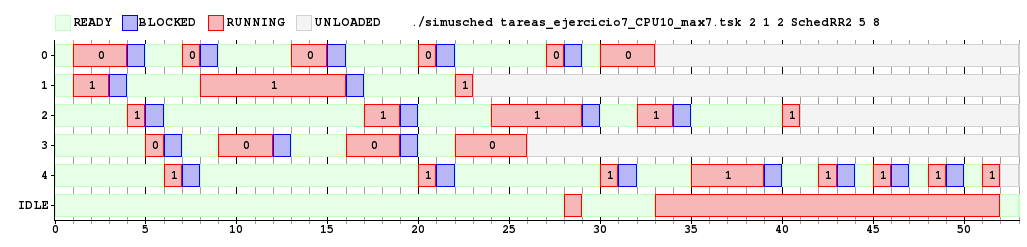
\includegraphics[width=450pt]{./figs/ej8/ej8-c2-q5-8.png}
\end{figure}

\indent De aquí se extrae que, para este lote de tareas, a partir de un quantum igual a cuatro para el core 0, y un quantum igual a 8 para el core 1 se obtiene la misma forma de ejecución si se aumentan los quantums.

\subsubsection{Tres cores}

\indent Análogamente al caso de estudio con 2 cores, se estudiaron casos con los mismos valores de quantum para los tres cores con quantums desde dos hasta diez y se volvió a analizar el turnaround time y el waiting time. A continuación se presentan gráficos para algunos casos:\\ 

\begin{figure}[h]
\centering                                                       
	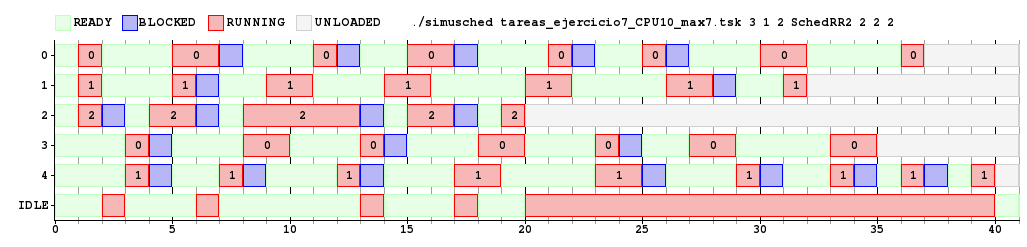
\includegraphics[width=450pt]{./figs/ej8/ej8-c3-q2.png}
\end{figure}

\begin{figure}[h]
\centering                                                       
	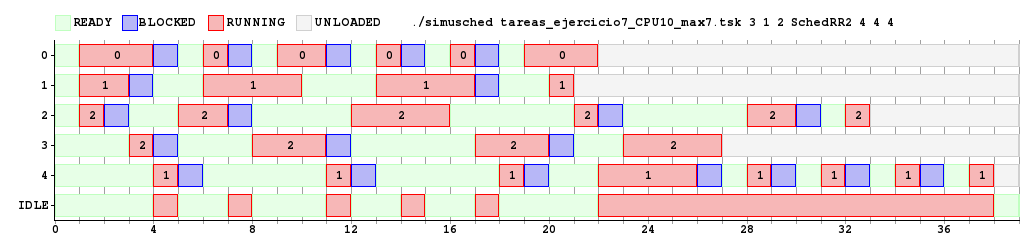
\includegraphics[width=450pt]{./figs/ej8/ej8-c3-q4.png}
\end{figure}

\clearpage

\indent De estos primeros dos gráficos podemos observar como se mejora el tiempo de ejecución para el caso de quantum igual a cuatro con respecto al de quantum igual a 2.\\
\begin{figure}[h]
\centering                                                       
	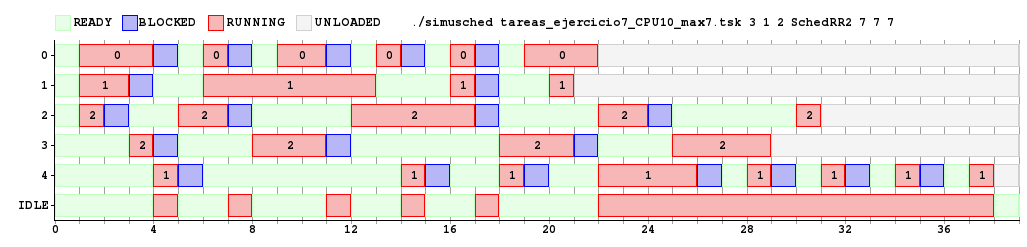
\includegraphics[width=450pt]{./figs/ej8/ej8-c3-q7.png}
\end{figure}

\begin{figure}[h]
\centering                                                       
	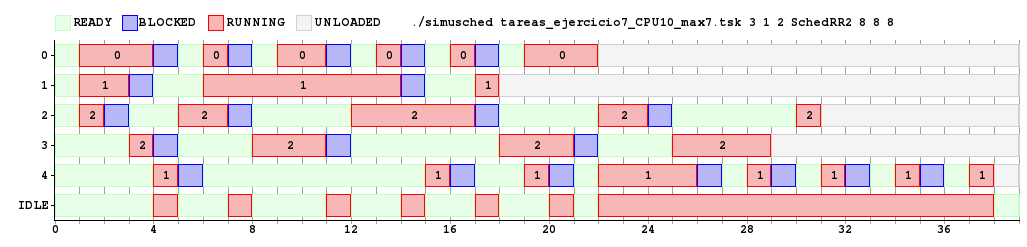
\includegraphics[width=450pt]{./figs/ej8/ej8-c3-q8.png}
\end{figure}

\begin{figure}[h]
\centering                                                       
	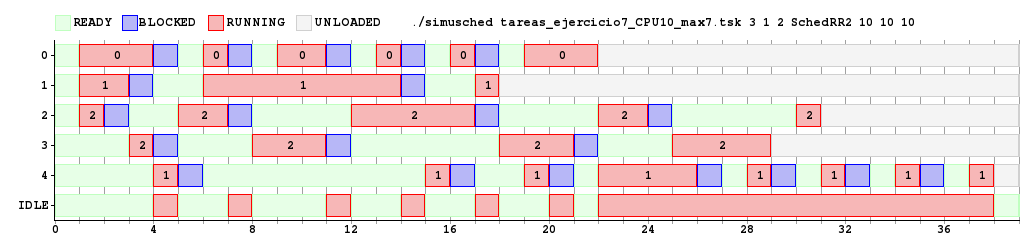
\includegraphics[width=450pt]{./figs/ej8/ej8-c3-q10.png}
\end{figure}

\clearpage

\indent Aquí podemos observar como si bien no se mejora el tiempo total de la ejecución de todas las tareas con respecto al caso con quantum igual a cuatro, si se mejora el de algunas de las tareas que tardan menos en ejecutarse. De la misma manera que en los anteriores casos de estudio, se observa como desde un quantum igual a ocho para los tres cores no varía ni la forma ni el tiempo de ejecución de las tareas.\\

\indent A partir de los casos analizados se generaron gráficos que muestran la variación del turnaround time y del waiting time para las tareas a medida que se aumenta el quantum para los tres cores.\\

\begin{figure}[h]
\centering                                                       
	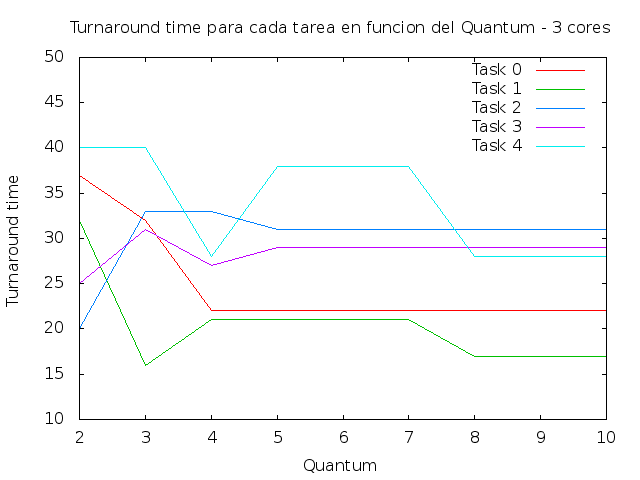
\includegraphics[width=300pt]{./figs/ej8/turnaround3cores.png}
\end{figure}

\begin{figure}[h]
\centering                                                       
	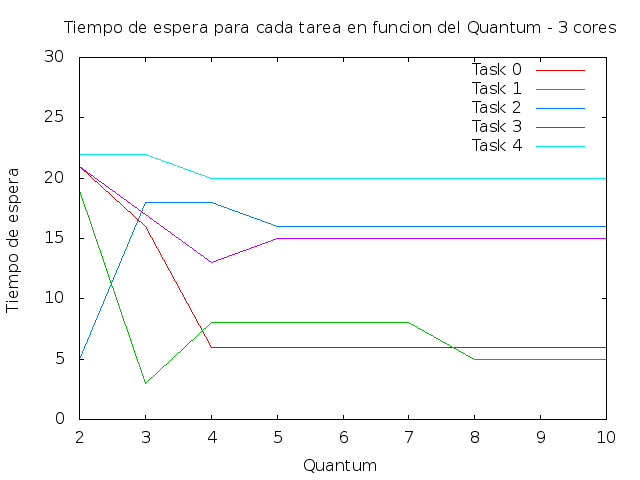
\includegraphics[width=300pt]{./figs/ej8/waitingtime3cores.png}
\end{figure}
\clearpage


\indent De estos gráficos se observa que a pesar de empezar de manera fluctuante, el turnaround time y el waiting time de las tareas se estabiliza a medida que se aumenta el quantum, para algunas antes que para otras.\\


\indent Para el análisis con distintos quantums en cada core, se procedió de la misma manera que cuando estudiamos los casos con dos cores. Los gráficos que se obtuvieron son:\\

\begin{figure}[h]
\centering                                                       
	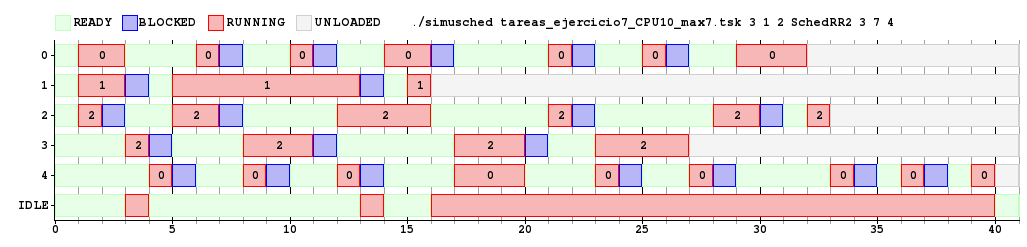
\includegraphics[width=450pt]{./figs/ej8/ej8-c3-q3-7-4.png}
\end{figure}

\begin{figure}[h]
\centering                                                       
	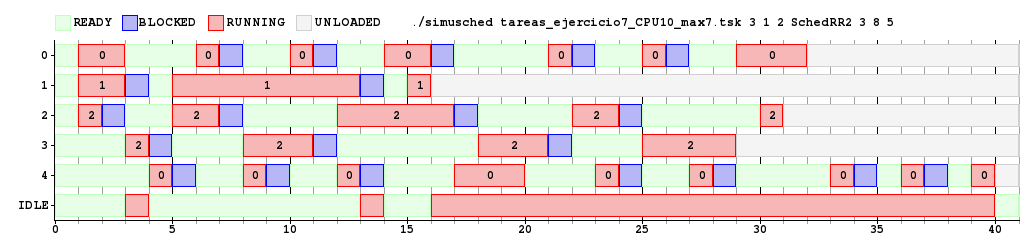
\includegraphics[width=450pt]{./figs/ej8/ej8-c3-q3-8-5.png}
\end{figure}

\begin{figure}[h]
\centering                                                       
	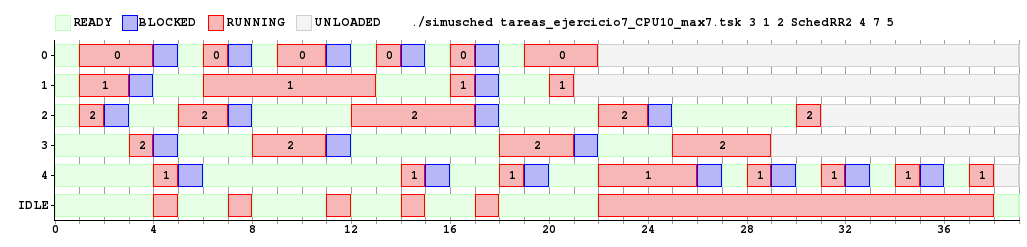
\includegraphics[width=450pt]{./figs/ej8/ej8-c3-q4-7-5.png}
\end{figure}

\begin{figure}[h]
\centering                                                       
	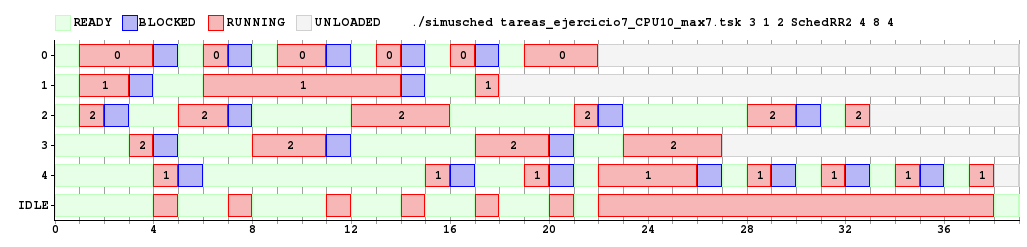
\includegraphics[width=450pt]{./figs/ej8/ej8-c3-q4-8-4.png}
\end{figure}

\begin{figure}[h]
\centering                                                       
	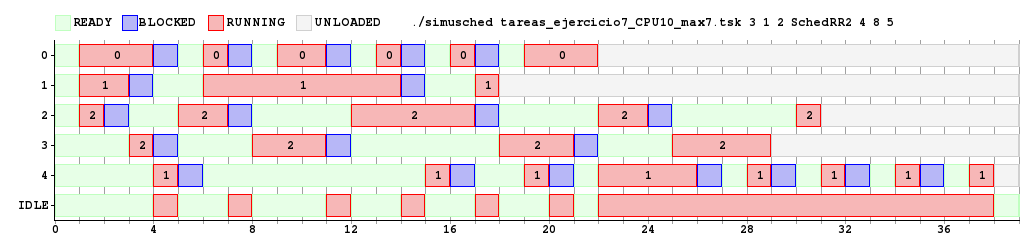
\includegraphics[width=450pt]{./figs/ej8/ej8-c3-q4-8-5.png}
\end{figure}

\clearpage

\indent De estos gráficos podemos observar como la manera en la que actúa cada core parece estabilizarse para cada uno por separado. De esta manera, el caso con quantum igual a cuatro para el core 0, quantum igual a 8 para el core 1 y quantum igual a 5 para el core 2, se nota que el scheduler se comporta de la misma manera que si los tres cores tuvieran quantum igual a ocho, que es el caso desde el cual observamos que se estabilizaba.\\
\indent Es decir que para este lote de tareas, a partir de un quantum igual a 4 para el core 0, un quantum igual a 8 para el core 1 y un quauntum igual a 5 para el core 2 el schedule se comportará de la misma manera.\\

\clearpage

\subsection{Comparación con los criterios del ejercicio 7}

\begin{figure}[h]
	\centering                                                       
	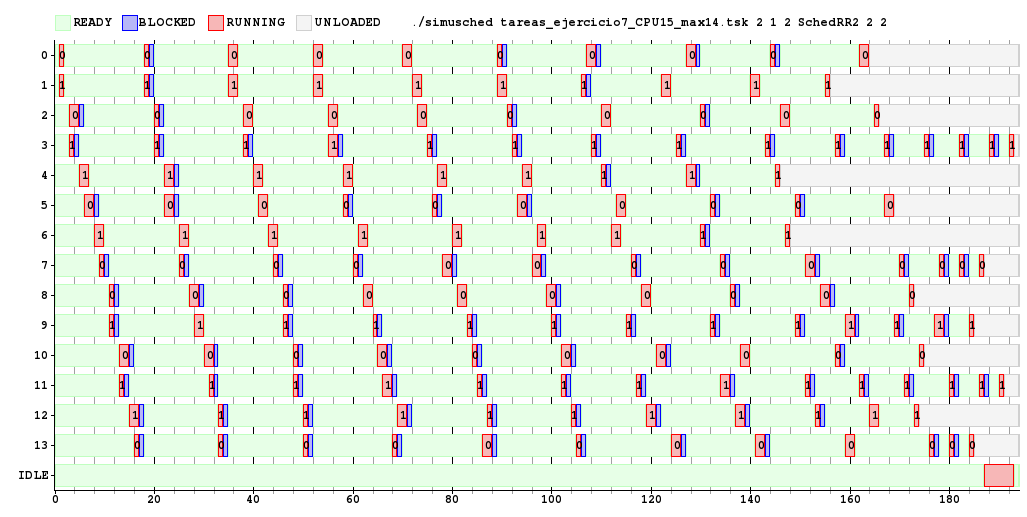
\includegraphics[width=450pt]{./figs/ejercicio8_2cores_quantum2.png}
\end{figure}

Lo que podemos ver al comparar la implementación de \textit{Round Robin 2} a diferencia del ejercicio 7, es que tenemos un algoritmo que no permite la migración de un proceso de un core a otro. Esto trae aparejado tanto ventajas como desventajas. En el primer grupo tenemos la ausencia del costo de migración entre núcleos, porque, lógicamente, dicha penalización no existe. En nuestras pruebas (con los costos de cambio de core y contexto fijados por el enunciado), esta ventaja es evidente cuando el quantum es pequeño, ya que la migración representa un porcentaje más alto de tiempo ``perdido'', en relación a la duración de cada turno para cada tarea. En nuestra experimentación en particular, se puede ver en el ejemplo de 2 cores, que baja el \textit{turnaround time} de aproximadamente 264 ticks a  198.\\
\indent Por otro lado, cuando el quantum no es pequeño, y los procesadores se utilizan de mejor forma, las tareas terminan de ejecutarse antes. Esto hace que la cantidad de veces que se cambia el núcleo de ejecución sean menos, haciendo que si eliminamos ese costo, no estemos mejorando de una manera tan importante el resultado final de la ejecución (es decir, estamos quitando algo que por otras características del experimento, ya no es tan protagonista de las mediciones como antes) como veremos a continuación.

\begin{figure}[h]
	\centering                                                       
	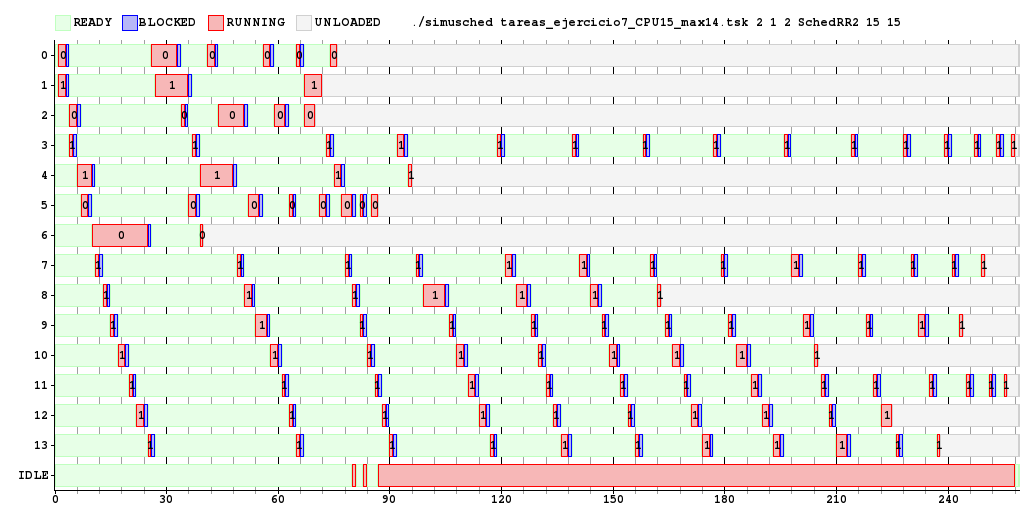
\includegraphics[width=450pt]{./figs/ejercicio8_2cores_quantum15.png}
\end{figure}

\clearpage

Las mejoras dadas por la falta de costo de migración de core no están presentes en el \textit{turnaround time}. No solo eso, sino que por el contrario, el \textit{turnaround time} es peor que en la experimentación con los mismos parámetros, pero con el algoritmo usado en el ejercicio 7.\\
\indent Esto es porque, como dijimos, no se aprovecha la fijación de una tarea con un core. El mayor problema con este enfoque es que uno no sabe de antemano cuanto va a tardar una tarea en terminar, y puede ser que mientras una tarea termina rápido, otra esté en estado \textit{ready}, atada a otro core, esperando su turno, mientras hay otro/s CPU/s en estado idle. Esto hace que el porcentaje de \textit{CPU Utilization} con este escenario disminuya de forma alarmante. Un CPU en estado idle existiendo tareas en estado \textit{ready} es una de las peores cosas que le pueden pasar a un algoritmo de scheduling como los que estamos viendo en este trabajo.

\subsubsection{Conclusiones de este ejercicio}

\indent Como conclusión, es claro que la elección del valor de los quantum para cada core es crucial para el desempeño del scheduler. Para los casos vistos existen valores de quantum a partir de los cuales la manera en la que se comporta el scheduler no cambia. \\
\indent Así, para el caso con un único core alcanza con elegir un quantum igual a 8. Para el caso con dos cores, basta con elegir un quantum igual a cuatro para el core 0, y un quantum igual a ocho para el core 1. Finalmente, para el caso con tres cores, elegir un quantum igual a cuatro para el core 0, un quantum igual a ocho para el core 1 y un quantum igual a 5 para el core 2 es suficiente para obtener los mejores valores de desempeño del scheduler.\\
\indent Nos quisiera mencionar además que la elección del quantum se ve fuertemente influencia por el lote de tareas que se corre. Es decir que no necesariamente estos valores de quantum serán los que mejor se comporten para otros lotes.\\

